\section{Electrical Design}
\subsection{Overview}
The 2021 year is our first year competing, so the electrical design of the robot focused on safety and reliability. The robot's electrical system is comprised of several modules that perform various tasks using custom PCBs with dedicated STM32 microcontrollers. The modules use the CAN bus to communicate with each other, and are made to be easily replaceable in case of failure. The robot can still function successfully if a module is disconnected. It also has several different safety features that increase reliability through redundancy.

\subsection{Power distribution}
The robot is powered using a single 12V 82Ah lead-acid battery. The type of battery we chose is used for electric power forklifts in the industry. The battery is designed to have a life of at least ten years. The voltage is stepped down or boosted as needed. Our nominal current consumption is calculated to be around 22 Amps when the robot moves at a rate of 5 MPH. The robot can operate continuously for 220 minutes using the 80Ah battery at the nominal current consumption rate. The battery has a recharge time of 24 hours. The robot was initially designed for the batteries to be hot-swapped, but the battery capacity has made that feature unnecessary. The power is distributed through Molex cables connected to every module with fuses for safety.
\subsection{Electronics Suite}

\subsubsection{Overview}
The robot has several modules and sensors throughout the system. The CAN bus allows devices to work independently, so if one device malfunctions, then the rest of the robot is functional.

\subsubsection{CAN molex}
We are using Molex connectors and cables to distribute power throughout the board. Each CAN Molex cable has six wires: 12V power, 5V power, ground, 3.3V E-stop signal, CAN high, and CAN low. The CAN Molex cable is an easy-to-route solution that provides a safe and reliable method to distribute power and data through the robot.

\subsubsection{Motor Control}
We use an STM32f103 microcontroller for our motor control. The calculated speed of each wheel is sent over the CAN bus, and the motor control board sets the speed of each wheel, respectively. Each set of wheels has an encoder that we use as feedback to control and correct the rate using a software PID controller on the STM32 chip.

\begin{figure}[h]
\centering
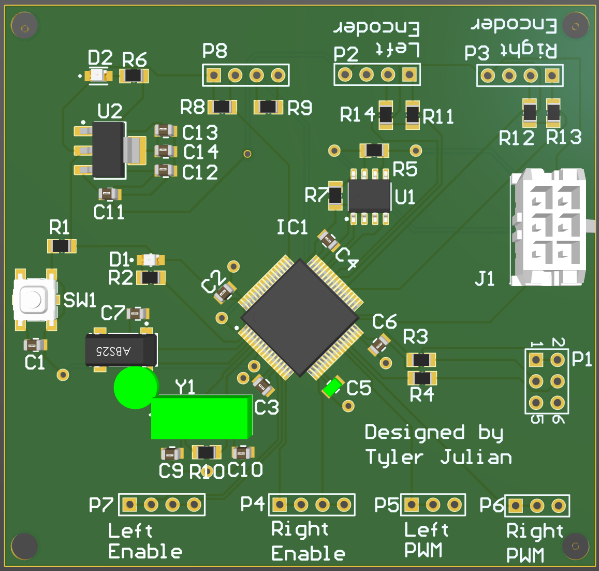
\includegraphics[width=0.3\textwidth]{images/electrical/motorControl.PNG}
\caption{The motor control PCB with the CAN Molex and STM32f103 chip.}
\end{figure}

\subsubsection{GPS}
The PCB we designed for the GPS module is based upon an STM32 microcontroller architecture. The microcontroller receives serial data from the sensor and then transmits it via CAN to our onboard computer for processing.

\begin{figure}[h]
\centering
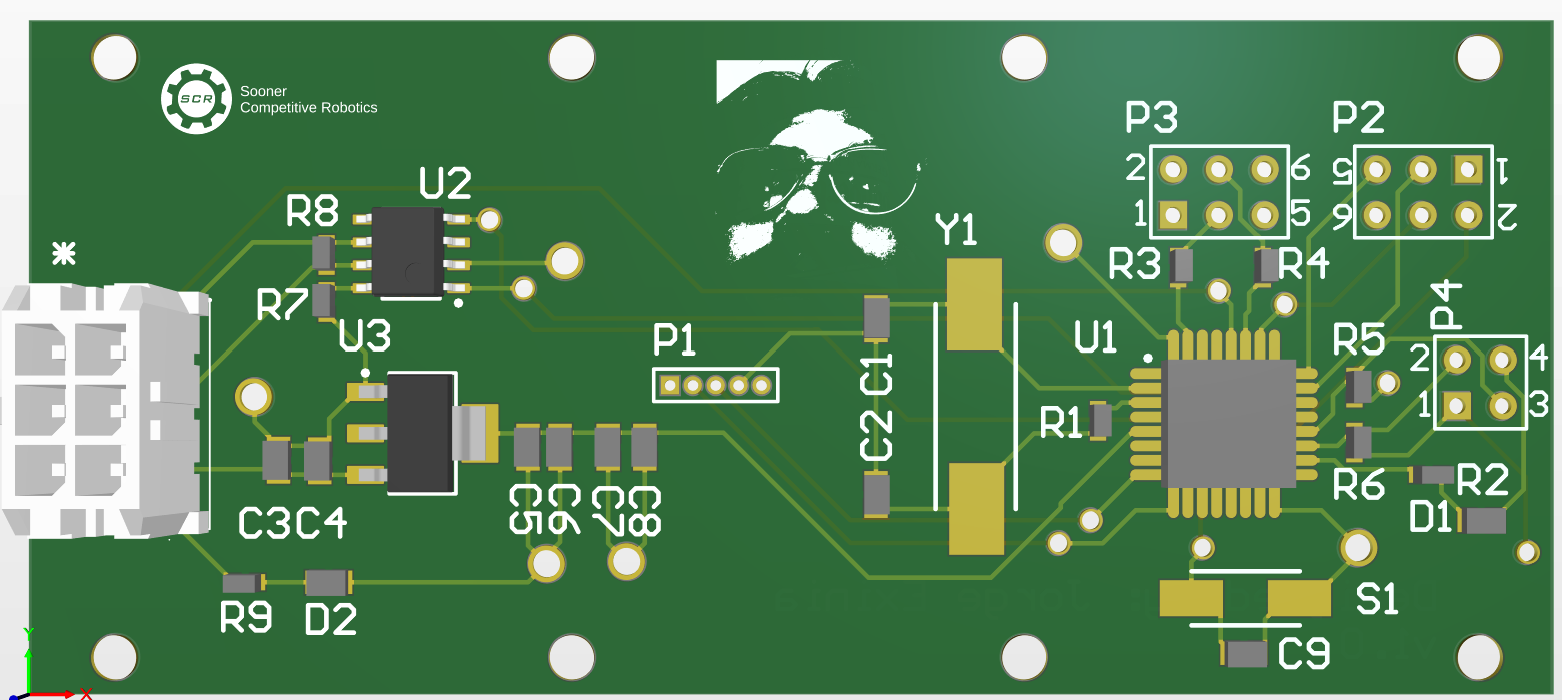
\includegraphics[width=0.3\textwidth]{images/electrical/gps.png}
\caption{The GPS PCB.}
\end{figure}

\subsubsection{Safety lights}
The PCB for the safety lights module is also based on an STM32 microcontroller architecture. An external 12V light is connected to the printed circuit board that is then switched on and off depending on the navigation state of the robot. This is done using a microcontroller and a MOSFET.

\begin{figure}[h]
\centering
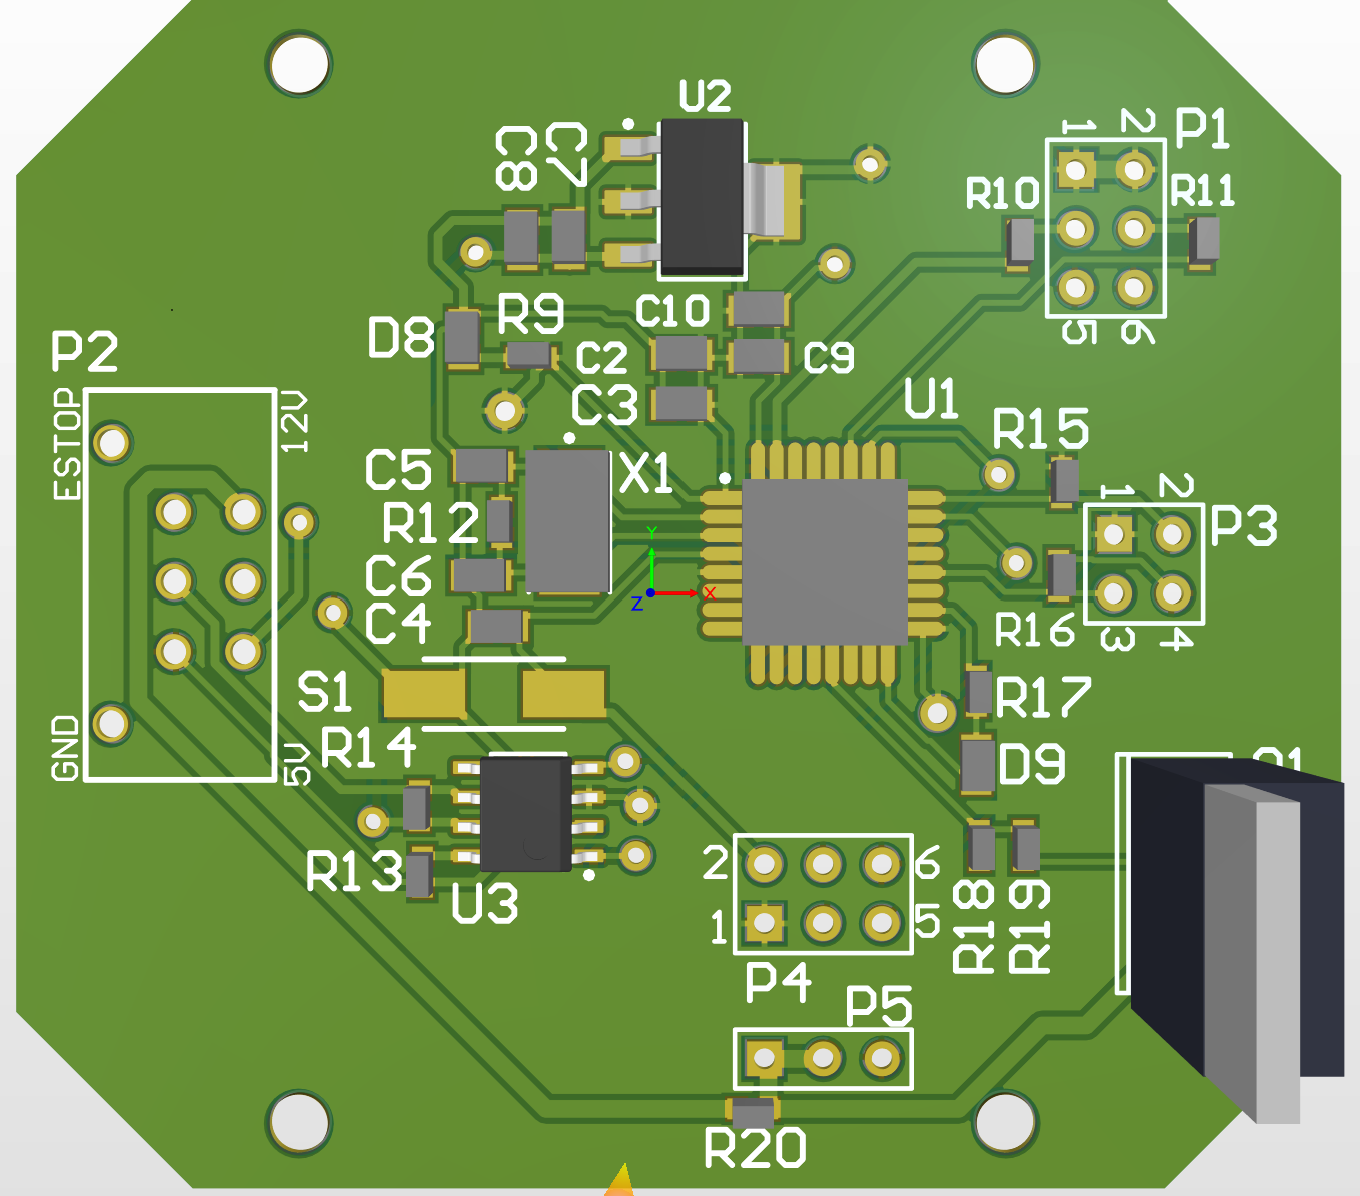
\includegraphics[width=0.3\textwidth]{images/electrical/SafetyLightsPCB.png}
\caption{The safety lights PCB.}
\end{figure}

\subsubsection{Remote E-stop}

Our remote E-stop system consists of two PCBs that communicate over radio to relay information about the E-stop and more. Each PCB uses an Adafruit Feather M0 LoRa as its microcontroller with a built-in radio transceiver for communication between the two. One PCB lies on the robot and waits for the E-stop radio signal. Once it receives the signal, the robot-wide E-stop signal is set, and the robot stops. The other PCB lies in a 3D printed remote control that will send the radio E-stop signal. The signal is sent with the press of the main button. Additionally, the remote also shows information about whether the robot is connected to the remote and acts as the start button to launch the robot into autonomous mode.

Both parts of the remote E-stop are constantly communicating, and if this connection is broken and a signal from the remote is not received after 2 seconds, E-stop will be initiated on the robot.

\begin{figure}[h]
\centering
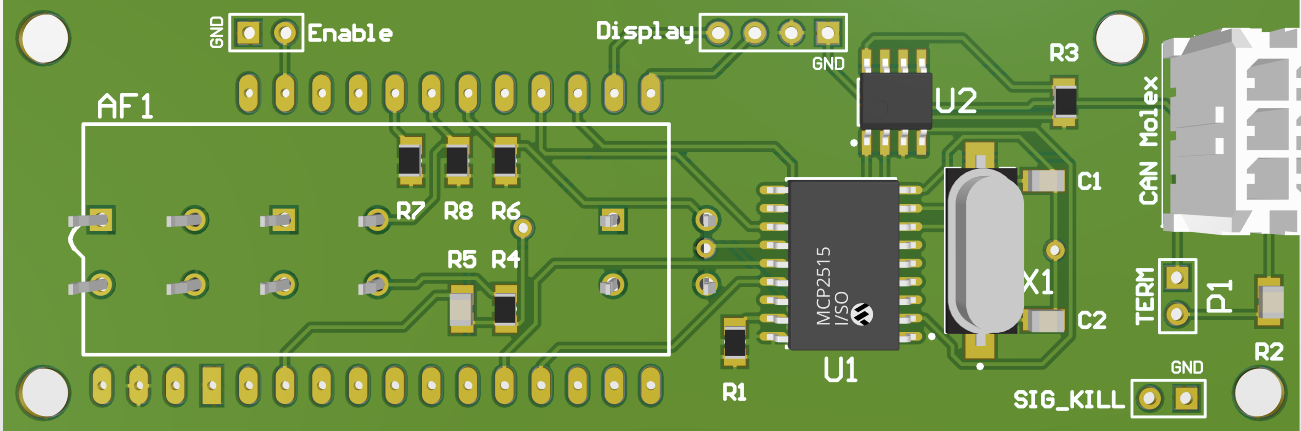
\includegraphics[width=0.3\textwidth]{images/electrical/estop.PNG}
\caption{The remote E-stop PCB.}
\end{figure}

\subsubsection{Hardware E-stop}
We convert the 3.3V E-stop signal to 24V to control an automotive contactor initially made for Toyota vehicles that cuts power to the motors when the E-stop signal is low or disconnected.

\subsubsection{IMU}
The Inertial Measurement Unit (IMU) is connected to the ODROID using USB. The ODROID processes the IMU data for use in our localization.

\subsubsection{LiDAR}
The LiDAR is connected to the ODROID using USB. The ODROID processes the LiDAR data and uses it for obstacle avoidance.

\subsubsection{Kinect}
We are using the X-Box Kinect 2 as a USB camera for our lane detection and other computer vision needs.

\subsection{Safety Devices}
\subsubsection{Emergency stops}
The robot has three ways to stop the robot:
\begin{itemize}
    \item a remote E-stop button
    \item a hardware E-stop button
    \item a key that cuts power to the entire robot when removed
\end{itemize}

The remote E-stop board generates a 3.3V E-stop signal that is sent through the entire robot. The robot is operational when the E-stop signal is high, but is not functional when the signal is low. The robot will shut down if it hasn't received a heartbeat message from the remote E-stop. The robot actively avoid obstacles using the LiDAR as well.

The robot has several systems that causes it to shut down for safety reasons. The first and most significant is the industrial contactor that cuts power to the motor controllers and motors when the E-stop signal is low. The second motor shutdown feature is a software stop that sets the motors speed to zero when the E-stop signal is low. The third feature isn't reliant on the E-stop signal. Emergency and mobility stop messages are sent through the CAN bus that disables the motors and sets the speed to zero. 

The three different systems make the robot safe and reliable with multiple layers of redundancy. 


\subsubsection{Safety Lights}
Our lights comply with the rules of competition. The lights remain solid when the robot is on and in manual mode, and strobe when the robot is autonomous. We use a 12V external light that is designed for semi-trucks and nighttime driving. With this in mind, there are not any visibility concerns.  The light is controlled with an STM32 microcontroller and a MOSFET. The MOSFET is rated for up to 50 Amps, which exceeds the current draw of the light.  

